\chapter{Dostupná řešení}


Cílem této kapitoly  je provést průzkum dostupných řešení pro animaci na stránkách s~cílem zmapování dostupné funkcionality. U~různých formátů se sledují tyto vlastnosti:

\begin{itemize}
\item Použitelnost na mobilních zařízení
\item Kvalita a~plynulost animace
\item Datová velikost animace
\end{itemize}

Použitelnost na mobilních zařízení se zkoušela na Apple iPhone 6\cite{iphone5} a~Samsung Galaxy Trend Mini \cite{samsung}.


\section{Adobe Flash}

Adobe Flash\cite{flash} je komplexní nástroj, se kterým lze vytvářet velké aplikace v~prostředí webových prohlížečů. Má vlastní nástroj pro vytváření projektů Adobe Flash MX (obrázek \ref{fig:flash-ui}), ve kterém se celý program vytváří a~testuje. Na webovou stránku se umístí  speciální HTML\cite{html5video} objekt, který tento program použije pro vykreslení objektu.


\begin{figure}[h]
\centering
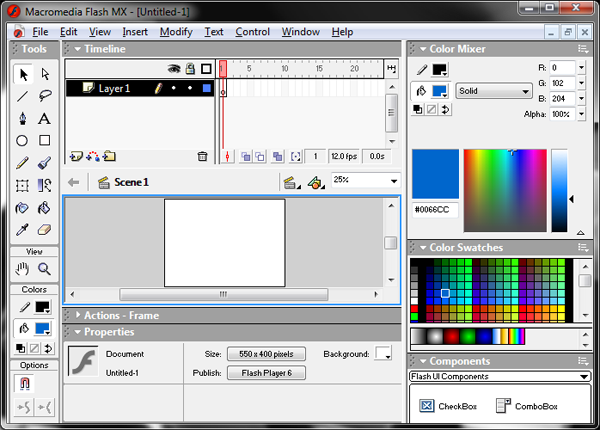
\includegraphics[width=0.8\textwidth]{./figures/flash-ui.png}
\caption{Prostředí programu Adobe Flash MX}
\label{fig:flash-ui}
\end{figure}



\subsection*{Vlastnosti}

Aplikace je volně ke stažení a~její použití je zdarma po získání bezplatné licence, k~vytváření aplikací je potřeba kromě prostředí znalost jazyka ActionScript\cite{ActionScript}, ve kterém se vytváří veškerá funkční logika. Projekt se musí nechat aplikací přeložit do souboru SWF\cite{swf}, který se potom vloží pomocí HTML\cite{html5video} elementu OBJECT na stránku. 

Prohlížeče návštěvníků stránky potom zavolají externí aplikaci, která tento SWF\cite{swf} soubor spustí a~zobrazí na stránce. Neřeší se pak v~tomto případě kompatibilní verze prohlížečů, ale verze externí apliace Adobe Flash\cite{flash}.

\begin{table}[h]\centering\footnotesize
	\caption[Kompatibilita Adobe FLash]{Kompatibilita Adobe Flash}\label{tab:research-flash}
	\begin{tabular}{|m{2.5cm}|m{2.5cm}|m{2.5cm}|m{2.5cm}|}\hline
		Internet Explorer & Gecko(Mozilla Firefox, Opera)	& WebKit (Safari, Google Chrome) &  Mobilní prohlížeče
		\tabularnewline \hline \hline 
		Ano od verze 6 &  Ano & Ano & Ne
		\tabularnewline \hline
	\end{tabular}
\end{table}


\subsection*{Zhodnocení}

Adobe Flash\cite{flash} je velmi rozšířený vzhledem k~velice bohatým možnostem interakce s~uživatelem a~zjednodušení pro testování mezi prohlížeči. Díky tomu je upředňostňovaný pro spoustu interakcí mezi uživateli. 

Hlavní nevýhoda je pak vysoká náročnost na výkon počítače, což se pak negativně projeví na výdrži baterie u~přenosných zařízení a~to i~u dobře optimalizované aplikace.  Další velkou nevýhodou je nedostatečná podpora v~mobilních zařízení\cite{mobile} v~dnešní době. 


\section{GIF}

GIF\cite{gif} je formát pro ukládání obrázků, který s~možností sekvence několika obrázků za sebou dokáže vytvořit animaci. V~průzkumu ho uvádím zejména pro to, že mnoho animací nebo krátkých videí se realizuje právě v~tomto formátu.

\subsection*{Vlastnosti}

Formát GIF\cite{gif} je používán pro grafiku s~malou paletou barev pro krátká videa nebo animace s~malým rozlišením. V~případě animace se ukládá každý krok v~animaci jako další obrázek. Kromě volby, zda se budou kroky animace opakovat nebo proběhnou pouze jednou, zde není žádná možnost ovládání. Grafika v~obrázku GIF je omezena na 256 barev, jedna z~nich je průhledná. Samotný obrázek je pak uložen bezztrátově, takže se často používá pro uložení jednoduše zbarvených firemních log.

\begin{table}[h]\centering\footnotesize
	\caption[Kompatibilita GIF]{Kompatibilita GIF}\label{tab:research-gif}
	\begin{tabular}{|m{2.5cm}|m{2.5cm}|m{2.5cm}|m{2.5cm}|}\hline
		Internet Explorer & Gecko(Mozilla Firefox, Opera)	& WebKit (Safari, Google Chrome) &  Mobilní prohlížeče
		\tabularnewline \hline \hline 
		Ano  &  Ano & Ano & Ano
		\tabularnewline \hline
	\end{tabular}
\end{table}

\subsection*{Zhodnocení}

Tento převážně obrázkový formát je málokdy používán k~nějakým ilustracím na webových stránkách. Je rozšířený hlavně kvůli jeho jednoduchosti při vytváření oproti jiným srovnávaným formátům. Návrh a~implementace této bakalářské práce dokáže formát GIF nahradit u~některých typových příkladů. 

Hlavní nevýhodou je omezené spektrum barev. Prohlížeče vykreslují GIF jako obrázek, takže se nedá nijak ovládat nebo nějak reagovat na uživatele. Naopak GIF formát je dostupný na všech používaných prohlížečích, takže se velice jednoduše integruje.


\section{HTML5 Video}

Moderní webové prohlížeče nám umožňují vkládat video přímo do prohlížeče. Tento způsob se používá pro přehrávání například na stránkách Youtube\cite{youtubeHtml5}. 
Video musí být uloženo v~přehratelném formátu MP4\cite{mp4}. Díky tomu prohlížeč dokáže začít přehrávat video nebo animaci, i~když ještě nemá stažený celý soubor.


\subsection*{Vlastnosti}

Video v~HTML5 se do webové stránky vkládá jako  HTML\cite{html5video} element, ve kterém se uvede cesta k~MP4\cite{mp4} souboru a~další parametry (například velikost objektu na stránce). Tento element je pak ve struktuře HTML, díky tomu aktivně dokáže komunikovat pomocí Javascriptu\cite{javascript}. To znamená, že se dá veškeré ovládání velice jednoduše řešit v~nativních knihovnách prohlížeče. 


\begin{table}[h]\centering\footnotesize
	\caption[Kompatibilita HTML5]{Kompatibilita HTML5 Video}\label{tab:research-html5}
	\begin{tabular}{|m{2.5cm}|m{2.5cm}|m{2.5cm}|m{2.5cm}|}\hline
		Internet Explorer & Gecko(Mozilla Firefox, Opera)	& WebKit (Safari, Google Chrome) &  Mobilní prohlížeče
		\tabularnewline \hline
		9.0+  &  Ano & Ano & Částečná (pouze režim přes celou obrazovku)
		\tabularnewline \hline
	\end{tabular}
\end{table}

\subsection*{Zhodnocení}

Tento formát je určen pro přehrávání videí a~filmů z~reálného prostředí. Animace na stránkách jsou předem připraveny digitálně. Problémem je funkčnost na mobilních zařízení, kde se HTML5 video přehrává na celé obrazovce\cite{html5VideoSupport}. Pokud nám jde pouze o~video, jeví se toto jako nejlepší cesta. 

Mnohdy je ale tato technologi používán jako grafické doplnění stránky\cite{effectHtml5}. Momentálně na mobilních zařízení často dochází k~nekorektnímu zobrazení nebo znepřístupnění webové stránky.

Pokud bychom pomocí HTML5 videa řešili některé animace, budeme postrádat průhlednost a~spoustu procesů pro přípravu videa. Tento formát není pro animace na stránkách určený.

\section{Zhodnocení}

Všechny formáty, které byly představeny, vypadají na první pohled dostačující, ale může se stát, že se požaduje na webových stránkách animace, která bude fungovat stejně v~IE8 nebo na mobilních zařízení. Pak by požadavkům nevyhovoval žádný z~jmenovaných formátů. 

\begin{table}[h]\centering\footnotesize
	\caption[analysisResult]{Zhodnocení současných formátů}\label{tab:research-result}
	\begin{tabular}{|l||m{2.5cm}|m{2.5cm}|m{2.5cm}|}
	\hline
		Formát & Ovladatelnost (Javascript) & Podpora mobilních zařízení & Minimální verze IE
		\tabularnewline \hline \hline 
		Adobe Flash  &  Ano & Ne & IE6+ \\ \hline
		HTML5 Video  &  Ano & Částečná & IE9+ \\ \hline
		GIF  &  Ne & Ano & Všechny současné
		\tabularnewline \hline
	\end{tabular}
\end{table}

Současné možnosti vytváření animací na webových stránkách jsou postačující pokud je možnost vynechat některý z~nepodporovaných požadavků v~tabulce \ref{tab:research-result}. 

V této práci je v~následujících kapitolách popsán a~vytvořen takový formát, aby splňoval všechny požadavky, které ostatní formáty nepodporují:

\begin{itemize}
\item Podpora prohlížečů od verze Internet Explorer 8+
\item Stejné chování na všech mobilních zařízení.
\item Podpora ovládání pomocí jazyka Javascript
\end{itemize}

